

%
% 1. Motivation / Goal
%   Why do you care about a debugger?
%   1.1. Fix bugs faster
%   1.2. Understand programs better
%   Why do you care to know how it's made?
%   1.3. It's typically not well understood, and it's cool.
%
% 2. Usefulness -- Live demo
%   2.0. Installation
%   2.1. Servant is a very good idea
%   2.1. Examples of where it's useful
%   2.2. Ditto
%   2.3. More examples..........
%
% 3. Look under the hood
%   3.0. System overview
%   3.1. GHC library directly, and its debugger
%   3.2. e.g. How do breakpoint works?
%   3.3. DAP -- GUI part
%   3.4. hie-bios
%

\documentclass{beamer}

\usetheme{welltyped}
\usepackage{hyperref}
\usepackage{tikz}
\usetikzlibrary{positioning}
\usetikzlibrary{shapes.geometric, arrows}

\tikzstyle{startstop} = [rectangle, rounded corners, minimum width=3cm, minimum height=1cm,text centered, draw=black, fill=red!30]
\tikzstyle{io} = [trapezium, trapezium left angle=70, trapezium right angle=110, minimum width=3cm, minimum height=1cm, text centered, draw=black, fill=blue!30]
\tikzstyle{process} = [rectangle, minimum width=3cm, minimum height=1cm, text centered, draw=black, fill=orange!30]
\tikzstyle{decision} = [diamond, minimum width=3cm, minimum height=1cm, text centered, draw=black, fill=green!30]
\tikzstyle{arrow} = [thick,->,>=stealth]

\begin{document}

\title{A modern step-through debugger for Haskell}
% \subtitle{A modern step-through debugger for Haskell}
\author{\textbf{Rodrigo Mesquita}\\Hannes Siebenhandl, Matthew Pickering}
\date{\today}
\maketitle

% \begin{frame}[fragile]
% \begin{verbatim}
%     break Main.hs 40
% \end{verbatim}
%
% \end{frame}
%
% \begin{frame}{My program has gone wrong...}
%     Consider this problem in your complicated code base...
% \end{frame}

% \begin{frame}{Functional Programming Myths}
%     \begin{itemize}
%         \item Strong types make tests unnecessary
%         \item A debugger is never needed in a functional language
%     \end{itemize}
% \end{frame}

% \begin{frame}{Familiar feelings?}
%
% \begin{itemize}
% \item "What exactly should I print...?"
% \item \textit{Paste}, \textit{Paste}, \textit{Paste} your println around the bug
% \item "Has that been evaluated?"
% \item "Which branch is taken here?"
% \item Waiting 10m for the compiler...
% \item "Where was this called?"
% \item \emph{"What the heck is my program doing?"}
% \end{itemize}
%
% % \begin{block}{Hiring us}
% % If you would like to enquire about working with us, please e-mail us at \href{mailto:info@well-typed.com}{info@well-typed.com}.
% % \end{block}
% \end{frame}

% \section{Yes, there's a better way}

% \begin{frame}{Yes, there's a better way}
%     \begin{itemize}
%         \item Find and fix bugs faster
%         \item Understand your program better
%     \end{itemize}
% \end{frame}

% \begin{frame} % {My not-so-secret agenda}
% \center
%
%     \emph{Convince you the Haskell debugger is worth your time}
%
%     % \pause The age of Haskell tooling is now!
%
%     % HLS is so much better, improving every day
%     % Profiling tools are getting so much better
%     % The age of tooling...!
%
%     % Convince you it is robust and industrial strength.
%     % That it will work without problems on your code base
%     % And that it will be useful
%     % Because we need bug reports
% \end{frame}


\begin{frame}{Motivation for a Haskell Debugger}
\begin{itemize}
    \item Find bugs!
    \item Interactively explore your code
    \item Understand Haskell and lazy evaluation
    \item Teach Haskell and lazy evaluation
\end{itemize}
\end{frame}

\begin{frame}{Live demo on example}
    % Live demo:
    % 1. Install hdb tool from hackage
    % 2. Install extension from Marketplace
    % 3. Create launch.json
    % 4. Run on simple file (pre-prepared)
    %   4.1 Show simple variables, expressions, step-line, step-in, step-out.
    % 5. Let's try something more complicated -- pandoc maybe?
    % 6. Break somewhere, show complex variables, print complicated expression
\begin{itemize}
\item Installation from scratch
    \begin{itemize}
        \item \texttt{cabal install haskell-debugger}
        \item Install "Haskell Debugger" VSCode extension
        \item \href{https://github.com/well-typed/haskell-debugger}{github.com/well-typed/haskell-debugger}
    \end{itemize}
% \item Configuring debugger options
\item Running to a breakpoint
    \begin{itemize}
        \item Create \texttt{launch.json}
    \end{itemize}
\item Varibles, evaluating expressions, stepping
    \begin{itemize}
        \item Stepping into thunk
    \end{itemize}
\end{itemize}
\end{frame}

\begin{frame}{Original design decisions~\footnote{S. Marlow et al. (2007) - A lightweight interactive debugger for Haskell}}
\begin{itemize}
\item Available by default, no recompilation needed
\item Does not hide the lazy evaluation model
    % -- \item Nor partly unevaluated data structures
    % \begin{itemize}
    %     \item Display unevaluated variable as thunks
    %     \item Step may jump to a thunk
    % \end{itemize}
\end{itemize}
\end{frame}

\begin{frame}{This is not a toy project!}
    \begin{itemize}
        \item Work funded by Mercury
        \item Uses GHC as a library (supports all extensions and flags)
            % \begin{itemize}
            %     \item thus supports all extensions and flags
            %     \item the 18yo GHCi debugger
            % \end{itemize}
        \item Uses DAP to support many editor clients
        \item Uses the same technology behind HLS to support complex projects and codebases
        \item \emph{It should just work}
    \end{itemize}
\end{frame}

\section{A look under the hood}

\begin{frame}{IDE integration: DAP}


    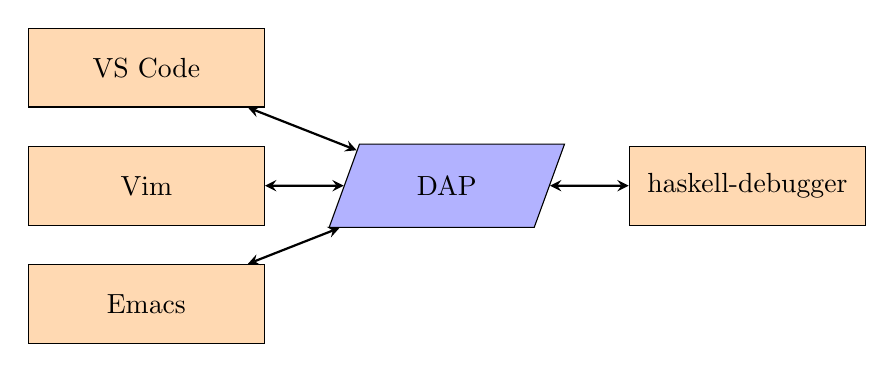
\begin{tikzpicture}[node distance=1cm]

        % Main DAP box
        \node[io] (dap) {DAP};

        % Debugger box on the right
        \node[process, right= of dap] (debugger) {haskell-debugger};

        % Editor boxes on the left
        \node[process, left= of dap, yshift=1.5cm] (vscode) {VS Code};
        \node[process, left= of dap] (vim) {Vim};
        \node[process, left= of dap, yshift=-1.5cm] (emacs) {Emacs};
        %
        % % Connections
        \draw[thick,<->,>=stealth] (vscode) -- (dap);
        \draw[thick,<->,>=stealth] (vim) -- (dap);
        \draw[thick,<->,>=stealth] (emacs) -- (dap);
        \draw[thick,<->,>=stealth] (dap) -- (debugger);

    \end{tikzpicture}
\end{frame}

\begin{frame}{The debugger process}
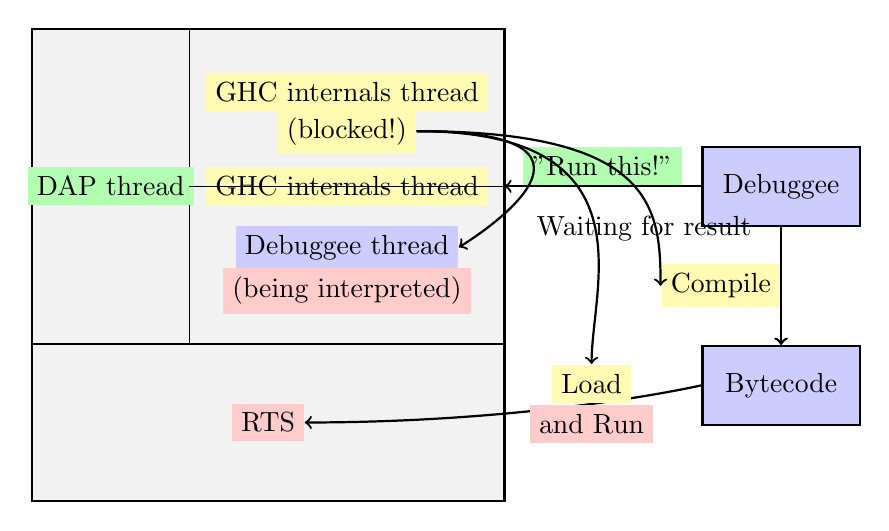
\begin{tikzpicture}
  % Draw main square
  \draw[thick, fill=gray!10] (0,0) rectangle (6,6);

  % Horizontal division (RTS at bottom)
  \draw[thick] (0,2) -- (6,2);

  % Vertical division (top part split)
  \draw (2,2) -- (2,6);

  % Labels inside
  \node[fill=red!20] (rts) at (3,1) {RTS};
  \node[fill=green!30] (dap) at (1,4) {DAP thread};
  \node<1-4>[fill=yellow!30] (internals) at (4,4) {GHC internals thread};
  \node<5->[fill=yellow!30, yshift=0.2cm] (internals) at (4,5) {GHC internals thread};
  \node<5->[fill=yellow!30, yshift=-0.3cm] (internals) at (4,5) {(blocked!)};

  % External node (Debuggee) as a box
  \node<2-4>[draw, thick, minimum width=2cm, minimum height=1cm,
        right=2.5cm of {(6,3)}, yshift=1cm, fill=blue!20] (debuggee) {Debuggee};

  \draw<2>[<-, thick] (6,4) -- (debuggee.west) node[midway, above, fill=green!30] {"Run this!"};

  % Bytecode node below Debuggee
  \node<3-4>[draw, thick, minimum width=2cm, minimum height=1cm,
        below=1.5cm of debuggee, fill=blue!20] (bytecode) {Bytecode};

  % Arrow from Debuggee to Bytecode
  \draw<3>[->, thick] (debuggee.south) -- (bytecode.north) node[midway, left, fill=yellow!30] (complabel) {Compile};

  \draw<3>[->, thick] (internals.east) .. controls +(3,0) and +(0,1) .. (complabel.west);

  \draw<4>[->, thick] (debuggee.south) -- (bytecode.north);
  \draw<4>[<-, thick] (rts.east) .. controls +(3,0) and +(0,0) .. (bytecode.west) node[midway, above, fill=yellow!30] (loadlabel) {Load} node[midway, below, fill=red!20] {and Run};
  \draw<4>[->, thick] (internals.east) .. controls +(3,0) and +(0,1) .. (loadlabel.north);

  % Vertical division for interpret debuggee
  \draw<5-> (2,4) -- (6,4);
  \node<5->[fill=blue!20, yshift=0.225cm] (interpret) at (4,3) {Debuggee thread};
  \node<5->[fill=red!20, yshift=-0.325cm] (interpreted) at (4,3) {(being interpreted)};

  \draw<5>[->, thick] (internals.east) .. controls +(3,0) and +(0,0) .. (interpret.east) node[midway, right, yshift=-0.5cm] {Waiting for result};

\end{tikzpicture}
\end{frame}

% case JUMP: int nextip = debuggee_bytecode[ip++];
%            ip         = nextip;
%            goto nextInst;
\begin{frame}[fragile]{Bytecode and the RTS interpreter}
\begin{verbatim}
debuggee_bytecode :: [Instr]

nextInst:
    let instr = debuggee_bytecode[ip++]
    switch instr:
        case ADD:   ...
                    goto nextInst
        case MUL:   ...
                    goto nextInst
        case JUMP:  ...
                    goto nextInst
        case PUSH:  ...
                    goto nextInst
\end{verbatim}
\end{frame}

\begin{frame}[fragile]{How to stop at a breakpoint?}
\begin{verbatim}
nextInst:
    let instr = debuggee_bytecode[ip++]
    switch instr:
        ...
        case BREAK:
            // A breakpoint instruction
\end{verbatim}
\end{frame}

\begin{frame}[fragile]{How to stop at a breakpoint?}
\begin{verbatim}
        case BREAK:
            if breakpoint is enabled:
                write data to shared memory;
                block on MVar
            else:
                goto nextInst
\end{verbatim}
\end{frame}

\begin{frame}{Stopped at a breakpoint}
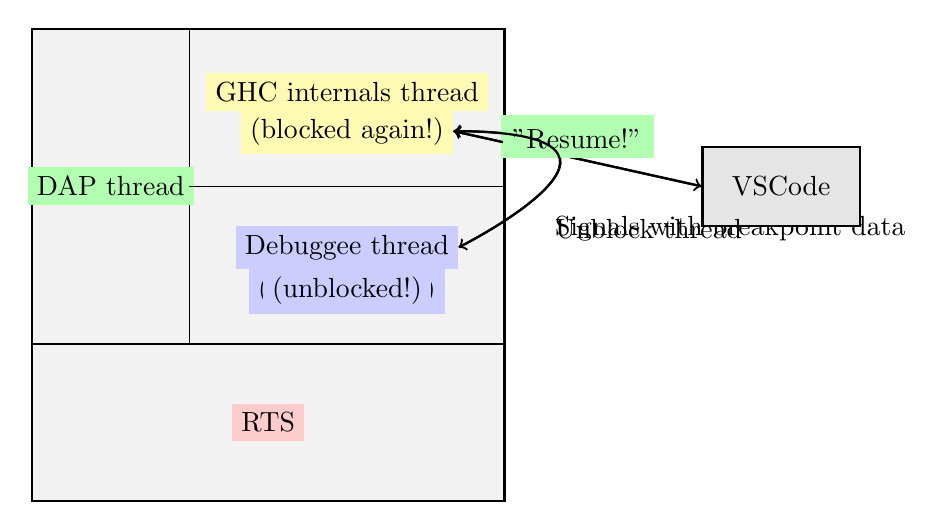
\begin{tikzpicture}
  % Draw main square
  \draw[thick, fill=gray!10] (0,0) rectangle (6,6);

  % Horizontal division (RTS at bottom)
  \draw[thick] (0,2) -- (6,2);

  % Vertical division (top part split)
  \draw (2,2) -- (2,6);

  % Labels inside
  \node[fill=red!20] (rts) at (3,1) {RTS};
  \node[fill=green!30] (dap) at (1,4) {DAP thread};
  \node[fill=yellow!30, yshift=0.2cm] (internals) at (4,5) {GHC internals thread};
  \node<1-3>[fill=yellow!30, yshift=-0.3cm] (internals) at (4,5) {(unblocked!)};
  \node<4>[fill=yellow!30, yshift=-0.3cm] (internals) at (4,5) {(blocked again!)};

  % Vertical division for interpret debuggee
  \draw (2,4) -- (6,4);
  \node[fill=blue!20, yshift=0.225cm] (interpret) at (4,3) {Debuggee thread};
  \node<1-3>[fill=blue!20, yshift=-0.325cm] (interpreted) at (4,3) {(now blocked!)};
  \node<4>[fill=blue!20, yshift=-0.325cm] (interpreted) at (4,3) {(unblocked!)};

  \draw<1>[<-, thick] (internals.east) .. controls +(3,0) and +(0,0) .. (interpret.east) node[midway, right, yshift=-0.5cm] {Signals with breakpoint data};

  \node<2-3>[draw, thick, minimum width=2cm, minimum height=1cm,
        right=2.5cm of {(6,3)}, yshift=1cm, fill=gray!20] (vscode) {VSCode};

  \draw<2>[->, thick] (internals.east) -- (vscode.west) node[midway, above, fill=green!30] {"Stopped!"};
  \draw<3>[<-, thick] (internals.east) -- (vscode.west) node[midway, above, fill=green!30] {"Resume!"};

  \draw<4>[->, thick] (internals.east) .. controls +(3,0) and +(0,0) .. (interpret.east) node[midway, right, yshift=-0.5cm] {Unblock thread};

\end{tikzpicture}
\end{frame}

\begin{frame}{Relating source code and bytecode}
\begin{itemize}
    \item Don't reverse engineer source from compiled code
    \item Annotate bytecode with source locations
    \item Reuses the tick mechanism used by HPC
    \item Robust wrt optimisations
\end{itemize}
\end{frame}

\begin{frame}{Breaking}
\begin{itemize}
    \item Enable breakpoints by source location
    \item Compare breakpoint instruction data against enabled locations
\end{itemize}
\end{frame}

\begin{frame}{Stepping}
\begin{itemize}
    \item Step-into
        \begin{itemize}
            \item Stop at immediate next break instruction
        \end{itemize}
    \item Step over
        \begin{itemize}
            \item Step-into/resume until stopped location matches current
        \end{itemize}
    \item Step out
        \begin{itemize}
            \item Walk stack to enable the breakpoint at the start of the continuation
            \item Ensure all continuations do have a breakpoint
            \item Challenge: compiled code vs. interpreted code
        \end{itemize}
\end{itemize}
\end{frame}

\begin{frame}{hie-bios / flag discovery}
    \begin{itemize}
        \item Delegate figuring out the flags to compile project to hie-bios
        \item Same tool used by HLS to configure project
    \end{itemize}
\end{frame}

\begin{frame}{Stack traces}
    \begin{itemize}
        \item All the information's on the stack
        \item How to decode it?
            \begin{itemize}
                \item -finfo-table-map
                \item interpreter continuations
            \end{itemize}
        \item What about tail calls?
        \item Binding stack frame variables
    \end{itemize}
\end{frame}

\begin{frame}{Exceptions}
    \begin{itemize}
        \item raise#
    \end{itemize}
\end{frame}

\section{Future}

\begin{frame}{Roadmap}
    \begin{itemize}
        \item Bug fixing (need reports!)
        \item Persistent Bytecode Artifacts
            \begin{itemize}
                \item Reduced startup time
                \item Step into library functions
                \item Better step-out
            \end{itemize}
        \item Backtraces (using existing mechanisms like IPE)
        \item Better exceptions support
        \item Better variables (more than just free vars in expr)
        \item Conditional breakpoints
        \item Disassemble requests
        \item Hot code reloading
        \item Multi-threaded debugging
        \item Compiled code debugging
        \item Time travelling debugging
    \end{itemize}
\end{frame}

% \begin{frame}{How can you help?}
%     \begin{itemize}
%         \item Bug reporting!
%         \item And bug fixing.
%         \item Plus lots of features missing!
%         \item Take a look at the issue tracker
%             \begin{itemize}
%                 \item From newcomer to expert-level tasks
%             \end{itemize}
%         \item \texttt{github.com/well-typed/haskell-debugger}
%     \end{itemize}
% \end{frame}

\end{document}
